
- from \textcite{cakp15}: The BR-FEM after Bernardi and Raugel \cite{bera85} is a modification of the P2P0 - FEM.
It is sometimes also called reduced $P_2\times P_0$ -FEM \cite{cakp15}

\textcite{bera85} (1985); 

\textcite{cakp15} (2015) state that this element also exists in 3D.

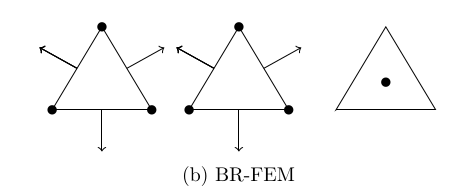
\includegraphics[width=5cm]{images/pair_bernardi_raugel/cakp15}

It is also mentioned in \textcite{bobf13} although it seems it is there called the SMALL element (p474).

In Lederer: "Consider the case d = 2. Above exam-
ple shows, that we only need to control the normal velocity at the edge, i.e. adding the
edge bubble for both components of the velocity seems to be sub optimal (with respect to
computational costs and the expected approximation properties). The idea now is to only
add the normal edge bubble."


